\documentclass[twocolumn,letterpaper, 12pt]{article}
\usepackage{import}
\usepackage{epa}
\usepackage{mlmodern}
\usepackage{amsfonts,amsmath,amssymb,amsthm}
\usepackage[left=.65in,top=.65in,bottom=.65in,right=.65in]{geometry}
\usepackage{lipsum} % to generate text
%%%%
%%%%
\usepackage[hidelinks]{hyperref}
\usepackage{caption}
\usepackage{csquotes}

\captionsetup{
	justification=justified,
	singlelinecheck=false
}
\captionsetup[figure]{
	width=\columnwidth
}
\captionsetup[figure*]{
	width=\textwidth
}
\captionsetup[table]{
	width=\columnwidth
}
\captionsetup[table*]{
	width=\textwidth
}
% Add Your packages here.


%%%%
%%%%
\title{Agricultural research on Refugia plants and rice pest control to farmland}

\author{%
\textbf{Rafli Harris Nasution{\textsuperscript{1}}, %
Eigen (Bui Gia Khanh){\textsuperscript{1}}} %
\\
\begin{small}
{\textsuperscript{1}}Draeigen Agricultural Laboratory \\ 
{\textsuperscript{*}}Correspondence: {formerly Hanoi University of Science, VNU} \\ 
\end{small}
}
\date{}
\begin{document}
\maketitle
%\linenumbers
%%%%%%%%%%%%%%%%%%%%%%%%%%%%%%%%%%%%%%%%%%%%%%%%%%%%%%%%%%%%%%%%%%%%%
% Abstract
%%%%%%%%%%%%%%%%%%%%%%%%%%%%%%%%%%%%%%%%%%%%%%%%%%%%%%%%%%%%%%%%%%%%%
\section*{Abstract}
This a research proposal for an experiment to measure the usefulness of refugia plants in driving away rice pests. For now, as far as this is a proposal in drafting, it is mainly a functioning document as both proposal forming and literature reviews. 
%%%%%%%%%%%%%%%%%%%%%%%%%%%%%%%%%%%%%%%%%%%%%%%%%%%%%%%%%%%%%%%%%%%%%
%%%%%%%%%%%%%%%%%%%%%%%%%%%%%%%%%%%%%%%%%%%%%%%%%%%%%%%%%%%%%%%%%%%%%
%%%%%%%%%%%%%%%%%%%%%%%%%%%%%%%%%%%%%%%%%%%%%%%%%%%%%%%%%%%%%%%%%%%%%
%%%%%%%%%%%%%%%%%%%%%%%%%%%%%%%%%%%%%%%%%%%%%%%%%%%%%%%%%%%%%%%%%%%%%
%%%%%%%%%%%%%%%%%%%%%%%%%%%%%%%%%%%%%%%%%%%%%%%%%%%%%%%%%%%%%%%%%%%%%
%%%%%%%%%%%%%%%%%%%%%%%%%%%%%%%%%%%%%%%%%%%%%%%%%%%%%%%%%%%%%%%%%%%%%
% Keywords: provide a list of 5 comma seperated keywords
%%%%%%%%%%%%%%%%%%%%%%%%%%%%%%%%%%%%%%%%%%%%%%%%%%%%%%%%%%%%%%%%%%%%%
\begin{EPAKeywords}
Refugia plant, pest control, arcology, agricultural technology, biological control. 
\end{EPAKeywords}
%
%%%%%%%%%%%%%%%%%%%%%%%%%%%%%%%%%%%%%%%%%%%%%%%%%%%%%%%%%%%%%%%%%%%%%
%%%%%%%%%%%%%%%%%%%%%%%%%%%% Introduction  %%%%%%%%%%%%%%%%%%%%%%%%%%
%%%%%%%%%%%%%%%%%%%%%%%%%%%%%%%%%%%%%%%%%%%%%%%%%%%%%%%%%%%%%%%%%%%%%
\section{Introduction}

This experiment is proposed by Rafli Harris Nasution, helped by Bui Gia Khanh. The research will primarily be done by Rafli (who has the farm land) alongside a couple of helpers (currently unspecified) to watch, help and report the progress of the experiment.

The paper itself, or the research that can be better expressed by the naming as \textbf{central topic} of: 
\begin{displayquote}
    Agricultural research on plant-based development and farming, for Refugia plants suitable in Indonesia for usage in rice plants pest control in context of Indonesia native ecological system and farmland. 
\end{displayquote}
Thus, many aspects of this research would be likely included and specified to be Indonesia-specific, though it is also very likely that it is only a very small part of what Indonesia many-island geography would suggest, land diversity. The following section and analysis would lay out the preliminary protruding ground that would matter most toward the project and research programme. 

\begin{figure}[htb]
    \centering
    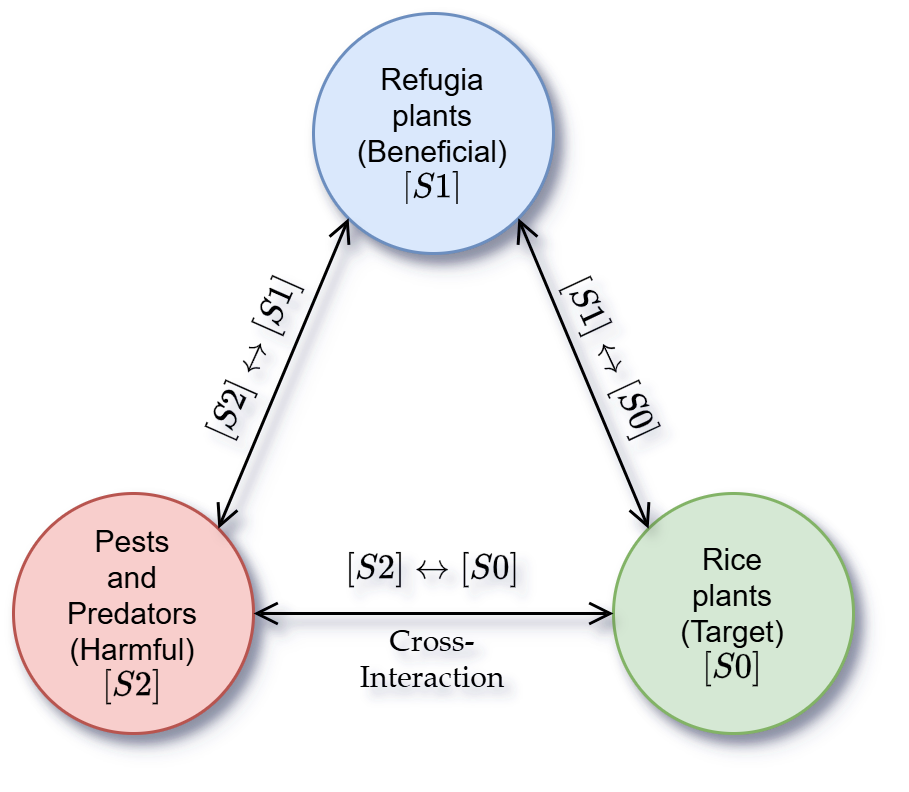
\includegraphics[width=\linewidth]{figure/cross_interaction.png}
    \caption{An example diagram for the interaction of three main target of interest - the harmful pest, the farmland with its crops, and the refugia plants i.e. the beneficial plants.}
\end{figure}

\subsection{Motivation}

Below is the motivation for this proposed experiment, which stems from also a wish for having scientific production, as well as formalizing a recent idea in development of an actual business as well as technology to reduce costs on actual farmlands. 
\begin{itemize}
    \item Experience: This experiment is primarily done to gain experience and establish the foundations of the members of this experiment in agriculture research and developments.
    \item Starting Point: This experiment also has the purpose of being a foundational experiment from which the research members can develop into other research and developments such as the processing of ingredients, making of pesticides and potentially eugenics.
\end{itemize}
\subsection{Prerequisite}
To do this experiment the researchers needs to have a foundational understanding of biology, agriculture, ecology and how they each influence each other and the means to applicate such knowledge into concrete results. The members of these experiment also needs to have some knowledge on how to do agriculture research of which they are sorely lacking in.

Furthermore, since this research utilize analysis and data processing as well as modelling, it is advisable to contain specific parts or skill set where data science, data processing, and \textbf{mathematical modelling} is available. 
\subsection{Proof of work}
Proof of work can be delivered in recorded results, procedures, data packages and analysis of the experimental and research progress. For data, we would have recorded topography of the entire research paper - the set up, environmental sensor information or initial starting point, analytical sensory information of relevant metrics; especially important is also the methodological procedures and processes in handling our methods, or plant solution. 
\subsubsection{Work Platform}
We will be working mainly on \textbf{Discord} for communication, with repositories, and data captured and stored within locked and private Cloudflare R2, or Blackblaze R2 storage option. When released or any workable software options and analysis, such would be placed in GitHub repository of the laboratory's organization category, respectively. 

Even though we mentioned Discord as our main communication channel, it is advised to note that in the future it might get updated to either migrate to different options, or changed entirely. However, in the middle-term of the consideration, Discord is still the main option of all. 

\subsection{Work, output and roles}
Currently, there are two (2) people of the newly formed research group. Either Draconite, who is mainly working as the field researcher, acting and operating on an actual farmland available, and Eigen, who is responsible mainly on the theoretical framework and analysis, data analysis and modelling of the system. Additionally, while it is said that Draconite is a field researcher, his expertise in biology contributes greatly to also the theoretical system of which will be developed during research. 

The \textit{expected research output} of this project is: 
\begin{itemize}
    \item A research paper about refugia plants and their effectiveness in this particular application. 
    \item Data and analysis (open source) on this particular research project. 
    \item Knowledge base, resources, and foundational documents set on this matter. 
\end{itemize}
Such would be the intended release. Additional releases can be considered charitable and is not forced to be there, hence there are no obligation to publish more than what is expected of here. 

Time commitment is awaiting from either side, as schedule and life situations dictates much of the concurrent decisions on profiling time and handling pipelines. However, should it be sufficient then it would be a continuous progress in multi-month successions. 
%%%%%%%%%%%%%%%%%%%%%%%%%%%%%%%%%%%%%%%%%%%%%%%%%%%%%%%%%%%%%%%%%%%%%
%%%%%%%%%%%%%%%%%%%%%%%%%%%%%%%%%%%%%%%%%%%%%%%%%%%%%%%%%%%%%%%%%%%%%
%%%%%%%%%%%%%%%%%%%%%%%%%%%%%%%%%%%%%%%%%%%%%%%%%%%%%%%%%%%%%%%%%%%%%
%%%%%%%%%%%%%%%%%%%%%%%%%%%%%%%%%%%%%%%%%%%%%%%%%%%%%%%%%%%%%%%%%%%%%
%%%%%%%%%%%%%%%%%%%%%%%%%%%%%%%%%%%%%%%%%%%%%%%%%%%%%%%%%%%%%%%%%%%%%
%%%%%%%%%%%%%%%%%%%%%%% Materials and Methods  %%%%%%%%%%%%%55%%%%%%%
%%%%%%%%%%%%%%%%%%%%%%%%%%%%%%%%%%%%%%%%%%%%%%%%%%%%%%%%%%%%%%%%%%%%%

\section{Research details}

For the research itself, it is also a dual process. Many parts of it would also be to learn, and to create custom and ground-up dissemination of agricultural research knowledge and frameworks. 

\subsection{Precursor question}

The research question at first is to see and find out if the presence of \textbf{refugia plants} can lower the amount of pests that can damage rice production and see if it would increase rice production. In details, if able, the main goal would be focused on: 
\begin{enumerate}
    \item Rice field cultivation: Can the presence of refugia plants, and to extends, the family of \textbf{beneficial ecosystem forming plants} that is not rice, to create a better microecology for rice, and to increase rice plants life, production rate, and quality? 
    \item Rice field pest control: Can the presence of refugia plants be a catalyst to prevent the accumulation and adverse effects seen of insects and plants? Can they be used to form the ecological barriers to prevent the intrusion of crop-destroying lucust, for examples, and else? 
    \item Alternative stream of products: Can refugia plants and its ecology creates alternative stream of products, residue, or any kind of profits if available? 
\end{enumerate}
These are the questions that will dictate the roles of the research itself. Benefits for it can be included as: 
\begin{enumerate}
    \item Lower manpower needed for farming and maintenance. 
    \item Lower or eliminate the cost of specific requisition of pesticide when farming. 
    \item Imrpove crop quality by minimizing pesticide usage. 
    \item Improve and harvest side products from the local microecosystem. 
\end{enumerate}
These are some important clarification and targets, as the research is funnelled and through dedicated pipeline for a private or at least commercial purpose bracket. Furthermore, it is also directly benefiting \textbf{small-scale farming} and micro-farming in a large farming structures, i.e. \textit{modular agricultural farming}. 
\subsection{Primary targets}

The primary targets contains several key figures and subject in the larger model of interest, and in a net of infrastructures, natural resources, and ecological targets as well as adversarial effects. 

\subsubsection{Refugia plants}

Refugia plants refers mostly to plants, micro-environments, or specific geological landscaping choices that provide on purpose, specific crop-friendly beneficial predator to weed out pests. Additionally, it is to provide shelters, survival and safety zone both from climate and environmental factors or conditions not specified, unknown but from known vectors and pressures, like evolutionary biology and ecological migration patterns. 

In sustainable farming and integrated pest management (IPM), refugia plants are companion flora grown around crops to harbour beneficial insects. By function, they provide a "refuge" (food, pollen, and shelter) for natural predators like ladybirds, hoverflies, and spiders, which naturally suppress agricultural pests.

Research into the utilities of refugia plants, refugia gardening and more are widely known, as seen in foundational literatures\cite{keppel2012refugia,morelli2016managing} as the introduction into the kind of `local climate control' method using refugia plants. Of the same foundational premise, evolutionary biology analysis and macro-ecological foundation for designing complex ecological simulations, and macro-biological populations dynamics are prominent at least in precursor materials\cite{abbott2000molecular,stewart2010refugia,tang2018identifying}, and their results are interesting: both as refugia applications in the harsh environment of Antartica, from 5D tracking (3D, time $t$, and cost $c$), to sustainment of plants in East Asia, shown credible progresses and validation on this method as one of the many way one can form closed or open ecological micro-biosphere to protect crops. As such, some moderate success in experimental and applied climate applications have been conducted, with moderate success\cite{baumgartner2018identifying,guim2024refugia}, and further progress as well as examples on this will have to be cataloged later during further reviews. 

On the topic of using refugia plants as micro-habitats and environmental isolation, biodiversity beneficiary, and overall 'biosphere engineering' for both protection and production increments, are various\cite{duff2024ecological,sijabat2026potential,mokoginta2022refugia,boinot2019alley,hardiansyah2021agrobiodiversity}, as can be seen in established literatures and known cases, though experiments and large-scale, time-series and long-term development analysis as well as registration remains to be seen, which is also our job. If not to say I have not found anything else rather than this, but this will do for the moment and the present. Though, it is fair to say most of these literatures are laboratory and ideal-condtion, fully controlled and high-tech environments with ample resources and logistics. Region-specific application also is a problem, as generalized framework for agricultural conditions classification rather than being \textbf{case-specific and geological specialization-locked} cases. We do not have money to test out all conditions and buy crops and fields all over the places. 

\subsection{Preliminary methodology}

The proposed preliminary methodology works as followed. We note that this is based on precursor information about the field, plot areas, plants, monitoring and so on. 

\begin{enumerate}
    \item Secure 4, $3\times 3$ plot to plant rice. Have a distance of at least $x$ meter between them so they don’t affect each other.
    \item Mark each plot with numbers, $F_1$ is the control field with no refugia plant, $F_2$ is the field with sunflower (insert species name idk, or $A$ arbitrary plant) plant, $F_3$ is the field with $B$ plant, and $F_4$ is the field planted with both $A$ and $B$ plant.
    \item Plant the rice and refugia plants according to each field’s marking.
    \item Check the bug population each week using the pitfall trap (what the hell is this draco) (Idk how this one works, need further research).
    \item Repeat until harvest. 
    \item Weight the harvest for each field. 
    \item Refine the data and evaluate methods, as well as creating plans. 
\end{enumerate}

There are factors unobserved here, and indeed there are many factors inside this pipeline that need fine tuning, including specific ways of determination of \textit{what to do, what to control, what to take care of} per each procedures. The issue with maintaining the ecosystem of refugia-rice synthesis is also not specified, and this is a direction worth analysing of. Maintenance and keeping control of the control group, as well as local-fauna penetration (near proximity might contaminate the control group or else), are some problems to note especially in the beginning of the work. Coordination and theoretical-experimental verification pipeline are not planned or designed, so we will have to deliberately focus on this edge since our work incorporates: 
\begin{itemize}
    \item A working theoretical framework of agricultural and ecological analysis. 
    \item A working set of simulations for control and identification/warning. 
    \item Finally a digital twin as well as a network of active control and manipulation, remote or on-field to control the field themselves alongside natural functions like refugia plants shield. 
\end{itemize}
So toward this end, we have plenty of work to refine this methodological area. 
\subsection{Measurements}

For now, initially, we have some plant for the \textit{measurement methodology without technology and only normal bookkeeping} - i.e. low-tech bookkeeping. At the end, of finite large time-step $t$, the precursor method is to analyze it via metric of predatory harmful insect population and rice production: 
\begin{itemize}
    \item Insect population is measured using a pitfall trap done at the [??? Week], [??? Week] and [??? Week]. The insect that is collected is first sorted out by their species and counted by hand in order to find out the insect population in each field.
    \item Rice production is measured by weighing the rice produced by each field ($F_1$, $F_2$, $F_3$ and $F_4$ respectively) and comparing them to each other.
\end{itemize}
Indeed, there are a lot of factors lacking. Because the lifetime and development time of rice plants are about \textbf{105 to 130 days}, this period can be analyzed in a much more detailed fashion. For example, one can try to supervise: 

\begin{enumerate}
    \item \textbf{Local fauna}: As stated, aside from the insect population $I_H$, there is the local insect fauna that protects rice plants from it, as $I_B$. Determining this, and monitoring the beneficiary contract as well as how this local fauna develops and add to the sustainment of nutritions and so on to the soil, is also a good thing. 
    \item \textbf{Soil analysis}: Soil sampling per 10-day or 5-day window is also advised as to see what kind of composition the soil takes, directly influences the plants themselves. Depending on if the rice plant are planted in \textbf{wet} or \textbf{dry} field, such would also change. 
    \item \textbf{Rice plant health}: Health analysis, basically, for quality too. 
    \item \textbf{Development timelines}: This is nice because even though refugia might proves beneficial, development timeline in details is also important in determining other features and other type of refugia support-modification (that is, modifying refugia plants shields for providing `personalized' care), if able. 
\end{enumerate}

There are also some issues, which would be nice to analyze though we do not know in which way and of what way. For example, while rice field requires this specific type of refugia arrangement, maybe other type of plants will have distinct ecological preference, thus making it unsuitable or with no additional improvement rather than not. To generalize this system further than just rice plant and even into strictly contained \textit{agricultural plants foundry} and grooming, a recommendation is also to develop along this line. 

That said, details are left later. Recently we also dabbled in the way of making Standard Operating Procedures (SOP), so we will have more on the way there. 

\subsubsection{Data analysis precursor}

The data that are collected by the researched is analyzed using two methods, first is the univariate analysis method which measures a variable’s quantity and frequency and the bivariate analysis method which measures the correlation between each variable. The bivariate analysis method that is used in this research is the [insert analysis method].

\section{Materials, Planning, and Methods}\label{sec:methods}

The research methodology strictly can be separated into two parts. First, theoretical and accumulation of research artifacts as well as experiences, procedures, SOP, and models, are to be conducted during the first few terms of the work. 

Below, is a diagram on how this paradigm operates in full. We do note that it is customary to note that it does not really entrench itself in the current form, and thus are required to be established into further modification when the project goes into operations. 

\clearpage

\section{Literature review}

To ground the research on comfortable evaluation ground, we are to provide a suitable place for deliberation and analysis of the project itself through real life examples and what current literature already established. While the outlook is good as current literature validates the premise of the research, further literature studies are there to help illustrates the grounding synthesis better, as well as the many challenges facing forward from what was known of other examples of the same kind. 

\clearpage

%%%%%%%%%%%%%%%%%%%%%%%%%%%%%%%%%%%%%%%%%%%%%%%%%%%%%%%%%%%%%%%%%%%%%%
% Example: Tabels
%%%%%%%%%%%%%%%%%%%%%%%%%%%%%%%%%%%%%%%%%%%%%%%%%%%%%%%%%%%%%%%%%%%%%%
%% To make a table full width in a two-column LaTeX layout, use the starred
%% environment table* (analogous to figure*). Put it near the top of a page
%% with [t] for best placement.

\section{Additional information}

Here goes additional information during drafting and research. 
%%%%%%%%%%%%%%%%%%%%%%%%%%%%%%%%%%%%%%%%%%%%%%%%%%%%%%%%%%%%%%%%%%%%%%
% Conflict of Interest: Templates (choose one and edit as needed)
%%%%%%%%%%%%%%%%%%%%%%%%%%%%%%%%%%%%%%%%%%%%%%%%%%%%%%%%%%%%%%%%%%%%%%
\subsection{Conflict of interest}
 %No conflict:
 The authors declare no conflict of interest.
%
\subsection{Sponsored research}
The study is being aimed for research funding grants. For now, key details on this are not given. 
% Sponsored research (sponsor had no role):
% This study received research funding from Company~X. The sponsor had no role in the
% study design, data collection, analysis, interpretation, or the decision to publish.
%
% Consulting/advisory role:
% Author~A serves as a paid consultant to Organization~Y. All other authors declare no
% conflict of interest.
%
% Employment:
% Author~B is employed by Company~Z. All other authors declare no conflict of interest.
%
% Equity ownership:
% Author~C holds equity in Company~X, which develops products related to this research.
% All other authors declare no conflict of interest.
%
% In-kind contributions:
% Seeds/feed/equipment were provided in kind by Company~X. The provider had no role in
% the study design, analysis, or manuscript preparation. The authors declare no other
% conflicts of interest.
%
% Patents / intellectual property:
% Author~A is an inventor on a patent application related to the methods described in this
% paper. All other authors declare no conflict of interest.
%%%%%%%%%%%%%%%%%%%%%%%%%%%%%%%%%%%%%%%%%%%%%%%%%%%%%%%%%%%%%%%%%%%%%%
%%%%%%%%%%%%%%%%%%%%%%%%%%%%%%%%%%%%%%%%%%%%%%%%%%%%%%%%%%%%%%%%%%%%%%
%%%%%%%%%%%%%%%%%%%%%%%%%%%%%%%%%%%%%%%%%%%%%%%%%%%%%%%%%%%%%%%%%%%%%%
\section{Author Contributions}
Author contribution are equal, though substantially so coming from Draco, or Rafli Harris Nasution for his contribution of experimental ground and resources, as well as his domain expertise in the matter of construction. 

Bui Gia Khanh would be contributing substantially on the wing of theoretical analysis, modelling, simulations, and computational optimization. 
%%%%%%%%%%%%%%%%%%%%%%%%%%%%%%%%%%%%%%%%%%%%%%%%%%%%%%%%%%%%%%%%%%%%%
\renewcommand\refname{References}
%%%%%%%%%%%%%%%%%%%%%%%%%%%%%%%%%%%%%%%%%%%%%%%%%%%%%%%%%%%%%%%%%%%%%
\begin{footnotesize}
\bibliographystyle{unsrt.bst}
\textnormal{\bibliography{references.bib}}
\end{footnotesize}

\end{document}